\documentclass{bioinfo}
\copyrightyear{2014}
\pubyear{2014}

\begin{document}
\firstpage{1}

\title[dnaplotlib]{dnaplotlib: a computational toolkit for the visualization of genetic constructs, libraries and associated data}
\author[Thomas E. Gorochowski \textit{et~al.}]{Thomas~E.~Gorochowski$^{1}$, Emerson~Glassey$^{1}$, Bryan~Der$^{1}$, D. Benjamin Gordon$^{1}$ and Christopher~A.~Voigt$^{1,}$\footnote{to whom correspondence should be addressed}}
\address{$^{1}$Department of Biological Engineering, Synthetic Biology Center, Massachusetts Institute of Technology, USA.}

\history{Received on XXXXX; revised on XXXXX; accepted on XXXXX}

\editor{Associate Editor: XXXXXXX}

\maketitle

\begin{abstract}

\section{Summary:}
dnaplotlib is a computational toolkit that enables highly customizable visualization of individual genetic constructs and libraries of design variants. Publication quality vector-based output is produced and all aspects of the rendering process can be easily customized or replaced by the user. dnaplotlib is capable of SBOL-compliant diagrams in addition to a format able to better illustrate the precise location and length of each genetic part. This alternative visualization method enables direct comparison with nucleotide-level information such as RNA-seq read depths. While it is envisaged that access will be predominantly via the programming interface, a web-based front-end is also provided to facilitate broader usage.

\section{Availability:}
dnaplotlib is cross-platform and open-source software developed using Python and released under the OSI recognised NPOSL-3.0 licence. Source code, documentation and a web front-end are available at the project website: \href{http://www.dnaplotlib.org}{http://www.dnaplotlib.org}.

\section{Contact:} \href{cavoigt@gmail.com}{cavoigt@gmail.com}
\end{abstract}

1 (1 para). Introduction to the need for standardized visualization of genetic designs. Sell the approach.

2 (1 para). Existing tools that are available and the current difficulties in using them, e.g., PigeonCAD. Why is it needed.

3 (3 para). What dnaplotlib is: Python-based, uses matplotlib, generates publication quality vector-based output. Highly customizable at all stages of the rendering process. Enables both single and libraries to be easily visualized. Describe the rendering pipeline (should tie into figure), and multiple types of output available.

4 (1 para). Web-based interface. What does this include, what it doesn't. Why did we make it.

5 (1 para). Broader view. How is this toolkit going to help the community. Broader use of SBOL-compliant figures? Easier communication of ideas. Still able to have a lab ``style'' to differentiate your work and emphasize aspects in unique ways.

\begin{figure*}[t]
\centering
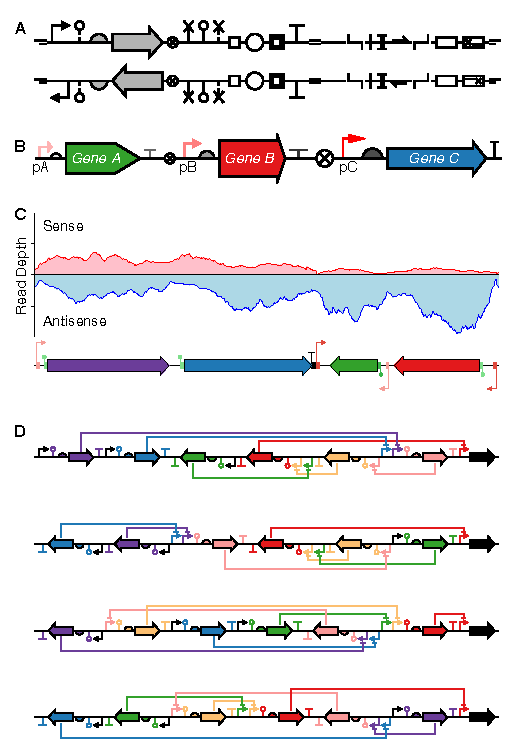
\includegraphics[width=\textwidth]{Figure1.pdf}
\caption{\label{fig:overview}Overview of dnaplotlib library and tools. (a) What can it produce, types of figure. (b) Potential usage of dnaplotlib (inputs, outputs). How it actually works.}
\end{figure*}

dnaplotlib is under continual development with a current focus on broadening the types of genetic element covered to include new areas of synthetic biology research, e.g., siRNAs. The project welcomes contributions from others within the community through the project website and public development repository at: \href{http://www.dnaplotlib.org}{http://www.dnaplotlib.org}.

\section*{ACKNOWLEDGEMENTS}
T.E.G. was supported by TO DO. E.G. was supported by TO DO. B.D. was supported by TO DO. C.A.V. was supported by TO DO.

\begin{thebibliography}{}
	
\bibitem[Nakao {\it et~al}., 2010]{Nakao10a} Nakao, N. and Mikhailov, S. (2010). Turing patterns in network-organized activator-inhibitor systems, {\it Nature Physics}, {\bf 6}, 544-550.

\bibitem[Gross {\it et~al}., 2008]{Gross08a} Gross, T. and Syama, H., editors (2008). {\it Adaptive Networks: Theory, Models and Applications.} Understanding Complex Systems. Springer, New York.

\bibitem[Mike {\it et~al}., 2014]{Mike14a} Mike's Nat. Biotech. paper.

\end{thebibliography}

\end{document}
